\documentclass[12pt]{article}
\usepackage[utf8]{inputenc}
\usepackage[T1]{fontenc}
\usepackage{lmodern}
\usepackage{geometry}
\geometry{margin=1in}
\usepackage{amsmath,amssymb}
\usepackage{enumitem}
\usepackage{xcolor}
\usepackage{hyperref}
\usepackage{listings}
\usepackage{listingsutf8}
\usepackage{tikz}

% --- Konfiguracja listings dla R (UTF-8 + polskie znaki) ---
\lstset{
  inputencoding=utf8,
  language=R,
  basicstyle=\ttfamily\footnotesize,
  backgroundcolor=\color{gray!10},
  frame=single,
  breaklines=true,
  keywordstyle=\color{blue},
  commentstyle=\color{teal},
  stringstyle=\color{brown},
  showstringspaces=false,
  literate=
    {ą}{{\k{a}}}1 {Ą}{{\k{A}}}1
    {ć}{{\'c}}1 {Ć}{{\'C}}1
    {ę}{{\k{e}}}1 {Ę}{{\k{E}}}1
    {ł}{{\l{}}}1 {Ł}{{\L{}}}1
    {ń}{{\'n}}1 {Ń}{{\'N}}1
    {ó}{{\'o}}1 {Ó}{{\'O}}1
    {ś}{{\'s}}1 {Ś}{{\'S}}1
    {ż}{{\.z}}1 {Ż}{{\.Z}}1
    {ź}{{\'z}}1 {Ź}{{\'Z}}1
    {–}{{-}}1
}

\title{Lekcja 7: Macierze dodatnio określone i rozkład Cholesky (R)}
\author{}
\date{}

\begin{document}
\maketitle

\begin{quote}
\emph{„Positive definite matrices are the natural habitat of least squares and energy.”}\\
Celem tej mini-lekcji jest \textbf{pomost} do rozkładów macierzowych: od definicji dodatniej określoności
do \textbf{rozkładu Cholesky} i zastosowania w rozwiązywaniu układów.
\end{quote}

\section*{Kontekst i cele}
\begin{itemize}
  \item Zrozumieć definicję: $A$ symetryczna dodatnio określona $\iff x^\top A x > 0$ dla $x\neq 0$.
  \item Rozpoznać praktyczne kryterium: \emph{wszystkie wartości własne dodatnie}.
  \item Umieć użyć \texttt{chol()} w R i zastosować do rozwiązywania układów $Ax=b$.
\end{itemize}

\section*{Zadanie 1. Sprawdzenie dodatniej określoności}
\textbf{Cel:} Sprawdź definicję na przykładzie i numerycznie.

\begin{lstlisting}
# a) Macierz symetryczna kandydat na PD
A <- matrix(c(4,1,1,
              1,3,0,
              1,0,2), nrow=3, byrow=TRUE)

# b) Wartości własne muszą być dodatnie
eig <- eigen(A)
eig$values
all(eig$values > 0)  # TRUE -> A jest dodatnio określona

# c) Test kwadratowy: x^T A x > 0 dla x != 0
set.seed(1)
x <- rnorm(3)
as.numeric(t(x) %*% A %*% x)
\end{lstlisting}

\section*{Zadanie 2. Kontrprzykład i intuicja}
\textbf{Cel:} Zobaczyć, co się psuje, gdy macierz nie jest PD.

\begin{lstlisting}
B <- matrix(c(0,1,1,
              1,0,1,
              1,1,0), nrow=3, byrow=TRUE)
eigen(B)$values        # uwaga na znaki
# Znajdź wektor x z x^T B x < 0 (np. spróbuj kilka losowych x)
set.seed(2)
xs <- replicate(10, rnorm(3))
apply(xs, 2, function(x) t(x) %*% B %*% x)
\end{lstlisting}

\section*{Zadanie 3. Rozkład Cholesky i weryfikacja}
\textbf{Cel:} Użyć \texttt{chol()} i sprawdzić rekonstrukcję.

\begin{lstlisting}
# chol() zwraca macierz górnotrójkątną L taką, że A = t(L) %*% L
L <- chol(A)
L

# Weryfikacja: t(L) %*% L powinno równać się A
t(L) %*% L
\end{lstlisting}

\noindent\textit{Uwaga:} \texttt{chol()} działa tylko dla macierzy SPD. Dla słabo PD (z bardzo małymi wartościami własnymi) może zgłaszać błąd z powodu niedokładności numerycznych.

\section*{Zadanie 4. Rozwiązywanie układu Ax=b przez Cholesky}
\textbf{Cel:} Porównać z \texttt{solve(A,b)} i zrozumieć dwa kroki: rozwiązać $L^\top y=b$, potem $Lx=y$.

\begin{lstlisting}
b <- c(1,2,3)

L <- chol(A)                    # A = t(L) %*% L
y <- forwardsolve(t(L), b)      # L^T y = b
x <- backsolve(L, y)            # L x = y
x

# Porównanie z "bezpośrednim" solve(A,b)
solve(A, b)
\end{lstlisting}

\section*{Zadanie 5. Jak generować macierze PD?}
\textbf{Cel:} Zobaczyć prosty generator SPD: $A=M^\top M$ (z pełnym rzędem).

\begin{lstlisting}
set.seed(123)
M <- matrix(rnorm(25), nrow=5)  # losowa macierz 5x5
A <- crossprod(M)               # A = t(M) %*% M  --> SPD
all(eigen(A)$values > 0)        # TRUE

# Cholesky i szybkie rozwiązywanie
b <- rnorm(5)
L <- chol(A)
x1 <- backsolve(L, forwardsolve(t(L), b))
x2 <- solve(A, b)
max(abs(x1 - x2))               # numerycznie bardzo mała różnica
\end{lstlisting}

\section*{Zadanie 6 (dla chętnych). Stabilność i quasi-PD}
\textbf{Cel:} Zbadać przypadki „bliskie” dodatniej określoności (małe wartości własne).

\begin{lstlisting}
# Macierz prawie PD: dodajemy małe zaburzenie do SPD
set.seed(7)
M <- matrix(rnorm(16), nrow=4)
A0 <- crossprod(M)
A_bad <- A0 - 1e-6 * diag(4)    # może stracić SPD numerycznie

# Spróbuj chol(); jeśli błąd, podnieś przekątną o małe "lambda"
try(chol(A_bad))
lambda <- 1e-5
A_fix <- A_bad + lambda * diag(4)
chol(A_fix)                     # powinno przejść

# Ćwiczenie: jak wpływa lambda na błąd rekonstrukcji i uwarunkowanie?
\end{lstlisting}


\section*{Geometria iloczynu skalarnego}

Każdy iloczyn skalarny w $\mathbb{R}^n$ można zapisać w postaci
\[
\langle x,y \rangle_A = x^\top A y,
\]
gdzie $A$ jest macierzą \emph{symetryczną dodatnio określoną (SPD)}.
Norma indukowana przez ten iloczyn skalarny to
\[
\|x\|_A = \sqrt{x^\top A x}.
\]

\textbf{Interpretacja geometryczna:} 
\begin{itemize}
  \item dla $A=I$ (macierz jednostkowa) kule $\{x : x^\top x = r^2\}$ są zwykłymi kołami w $\mathbb{R}^2$,
  \item dla ogólnej SPD $A$ zbiory $\{x : x^\top A x = r^2\}$ są elipsami (w $\mathbb{R}^2$) lub elipsoidami (w $\mathbb{R}^n$),
  \item osie elipsy odpowiadają wektorom własnym macierzy $A$, a długości półosi są odwrotnie proporcjonalne do pierwiastków z wartości własnych.
\end{itemize}

\begin{center}
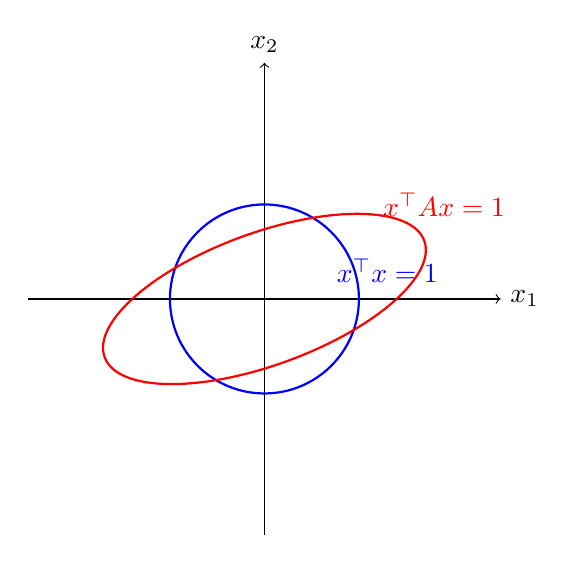
\begin{tikzpicture}[scale=1.2]
  % Osie
  \draw[->] (-2.5,0) -- (2.5,0) node[right] {$x_1$};
  \draw[->] (0,-2.5) -- (0,2.5) node[above] {$x_2$};

  % Okrąg jednostkowy (A = I)
  \draw[blue,thick] (0,0) circle (1);
  \node[blue] at (1.3,0.3) {$x^\top x = 1$};

  % Elipsa (A SPD)
  \draw[red,thick,rotate=20] (0,0) ellipse (1.8 and 0.7);
  \node[red] at (1.9,1.0) {$x^\top A x = 1$};
\end{tikzpicture}
\end{center}

\noindent
\textbf{Wniosek:} macierze SPD \emph{zmieniają metrykę przestrzeni} – kula euklidesowa staje się elipsą,
ale wciąż zachowujemy strukturę iloczynu skalarnego i normy.
Rozkład Cholesky $A=R^\top R$ pozwala wrócić do zwykłego układu współrzędnych,
gdzie elipsa staje się okręgiem.


\section*{English Corner (mini)}
\begin{quote}
\textbf{Positive definite (SPD) matrix:} a symmetric matrix $A$ with $x^\top A x > 0$ for all nonzero $x$.\\
\textbf{Cholesky factorization:} $A = R^\top R$ with $R$ upper-triangular (in R: \texttt{chol(A)}).
\end{quote}

\end{document}
